% ======================================================================
%  Quanser 2-DOF Serial Flexible Link  --  schematic (top view, horizontal
%  plane, gravity out of the page).
%
%  Serial elbow arm:
%    base --[motor 1 + harmonic drive]-- flexible link 1 --[motor 2 +
%    harmonic drive, the "elbow"]-- flexible link 2 -- tip mass.
%  Each thin spring-steel beam is modelled as a RIGID beam on a TORSIONAL
%  ROOT SPRING (Ks_i, base strain gauge); an encoder measures the joint
%  (hub) angle, a strain gauge the small elastic deflection.
%
%  compare_methods.py controls STAGE 1 only: joint 1 + link 1, with the
%  elbow + link 2 lumped as the link-1 end load (M12, J12).  Its 4-state
%  model is  x = [theta_h, theta_t, theta_h_dot, theta_t_dot],
%  output  y = theta_h + theta_t  (C_TIP = [1,1,0,0]).
%
%  Compile:  pdflatex model_diagram.tex
% ======================================================================
\documentclass[border=6pt]{standalone}
\usepackage{amsmath}
\usepackage{bm}
\usepackage{xcolor}
\usepackage{tikz}
\usetikzlibrary{arrows.meta,decorations.pathmorphing,angles,quotes,
                calc,positioning,bending,fpu,backgrounds}

% ---- palette ----------------------------------------------------------
\definecolor{hubcol}{HTML}{1f77b4}   % joint 1 (hub) / rigid direction
\definecolor{linkcol}{HTML}{2ca02c}  % flexible link 1
\definecolor{j2col}{HTML}{7b3294}    % joint 2 (elbow)
\definecolor{link2col}{HTML}{117777} % flexible link 2
\definecolor{tipcol}{HTML}{d62728}   % deflection / output
\definecolor{motcol}{HTML}{555555}   % motor
\definecolor{refcol}{HTML}{999999}   % reference axis
\definecolor{springcol}{HTML}{ff7f0e}% torsional stiffness Ks
\definecolor{stagecol}{HTML}{1f77b4} % Stage-1 highlight

\begin{document}
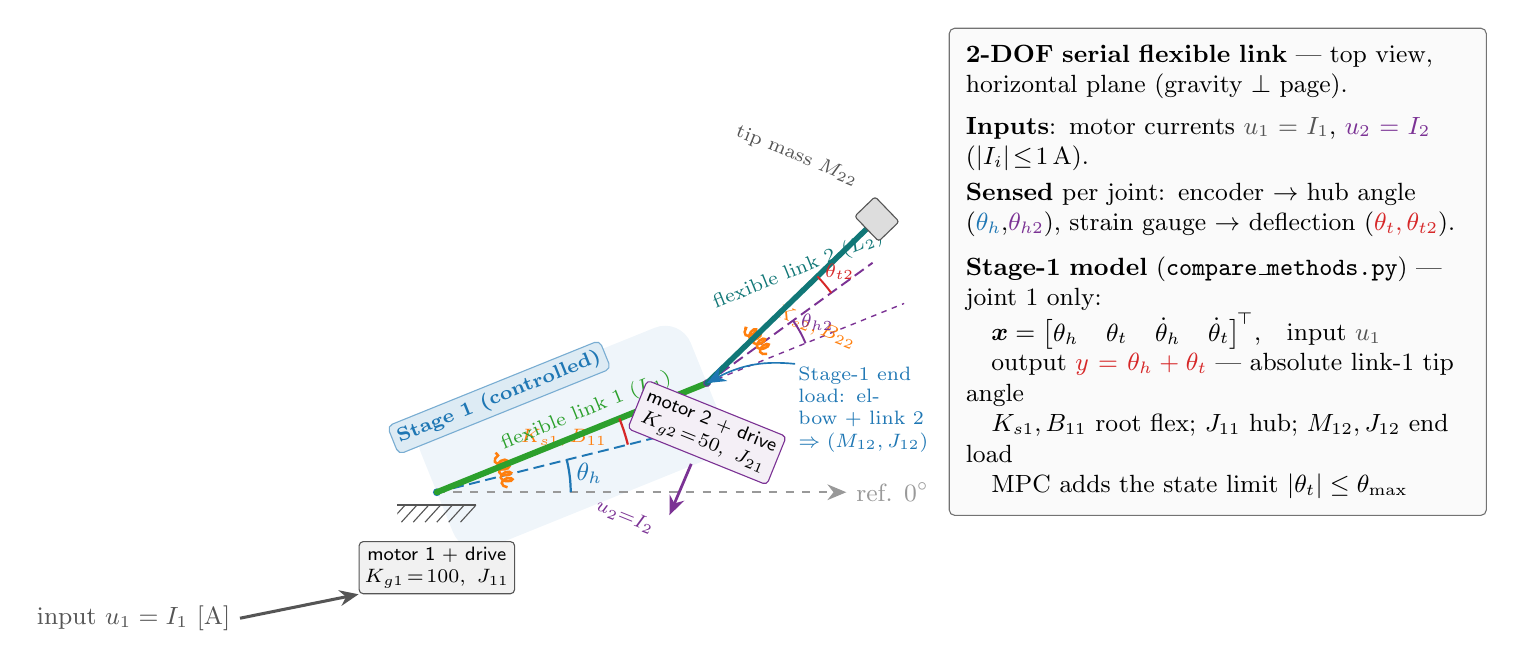
\begin{tikzpicture}[
    >={Stealth[length=2.4mm,width=2mm]},
    font=\small,
    spring/.style={springcol,line width=0.9pt,decorate,
        decoration={coil,aspect=0.55,segment length=2.2pt,amplitude=2pt}},
  ]

  % ---- joint-1 (base) geometry, degrees ------------------------------
  \def\hA{14}     % hub-1 angle (encoder, the joint position)   theta_h
  \def\aA{22}     % link-1 actual angle  -> deflection theta_t = aA-hA
  \def\lA{3.7}    % link-1 drawn length
  % ---- joint-2 (elbow) geometry, RELATIVE to link 1, degrees ---------
  \def\hBrel{14}  % hub-2 angle (encoder), relative to link 1
  \def\aBrel{22}  % link-2 actual angle, relative to link 1
  \def\lB{3.0}    % link-2 drawn length

  \coordinate (O1) at (0,0);
  \coordinate (E)  at (\aA:\lA);                 % elbow = link-1 tip

  % ====================================================================
  %  Stage-1 highlight band (behind everything): what compare_methods
  %  actually controls -- joint 1 + link 1.
  % ====================================================================
  \begin{scope}[on background layer]
    \fill[stagecol!7,rounded corners=10pt]
       ($(O1)+(\aA-90:0.9)$) -- ($(E)+(\aA-90:0.9)$)
       -- ($(E)+(\aA+90:0.9)$) -- ($(O1)+(\aA+90:0.9)$) -- cycle;
  \end{scope}
  \node[fill=stagecol!15,draw=stagecol!60,rounded corners=2pt,inner sep=2pt,
        font=\scriptsize\bfseries,text=stagecol,rotate=\aA,anchor=south]
        at ($(O1)!0.32!(E) + (\aA+90:0.62)$) {Stage 1 (controlled)};

  % ---- fixed reference axis (joint-1 zero) ---------------------------
  \draw[refcol,dashed,->,line width=0.6pt] (0,0) -- (5.2,0)
       node[right,refcol] {ref. $0^\circ$};

  % ---- fixed base / ground -------------------------------------------
  \begin{scope}
    \clip (-0.5,-0.5) rectangle (0.5,-0.16);
    \foreach \x in {-0.55,-0.4,...,0.55}
      \draw[motcol,line width=0.4pt] (\x,-0.16) -- (\x-0.2,-0.38);
  \end{scope}
  \draw[motcol,line width=0.8pt] (-0.5,-0.16) -- (0.5,-0.16);

  % ====================================================================
  %  JOINT 1  (motor 1 + harmonic drive)  -- hub, light inertia J11
  % ====================================================================
  \node[draw=motcol,fill=motcol!8,rounded corners=1.5pt,inner sep=2pt,
        font=\scriptsize\sffamily,align=center,anchor=north]
        (m1) at (0,-0.62) {motor 1 + drive\\$K_{g1}\!=\!100,\ J_{11}$};
  \draw[motcol,->,line width=1.1pt] (-2.5,-1.6) -- (m1.south west);
  \node[motcol,anchor=east,font=\small] at (-2.5,-1.6)
        {input $u_1=I_{1}$ [A]};

  % hub-1 commanded (rigid) direction
  \draw[hubcol,dash pattern=on 4pt off 2pt,line width=0.7pt]
        (O1) -- (\hA:\lA-0.2);
  \fill[hubcol] (O1) circle (1.4pt);

  % root torsional spring Ks1 + damper B11 (deflection exaggerated)
  \draw[spring] (\hA-10:0.9) arc (\hA-10:\aA+12:0.9);
  \node[springcol,font=\scriptsize,anchor=south west] at (\aA+4:1.05)
        {$K_{s1},B_{11}$};

  % flexible link 1 : rigid beam, rotated by the deflection about the root
  \draw[linkcol,line width=2.2pt,line cap=round] (O1) -- (E);
  \node[linkcol,font=\scriptsize,anchor=south,rotate=\aA]
        at (\aA:\lA*0.58) {flexible link 1 ($L_1$)};

  % theta_h (encoder) below the link, theta_t (strain) in the flex wedge
  \draw[hubcol,line width=0.8pt] (1.7,0) arc (0:\hA:1.7);
  \node[hubcol] at (\hA*0.5:1.95) {$\theta_h$};
  \draw[tipcol,line width=0.8pt] (\hA:2.5) arc (\hA:\aA:2.5);
  \node[tipcol] at ({(\hA+\aA)/2}:2.78) {$\theta_t$};

  % ====================================================================
  %  JOINT 2 (elbow) + LINK 2  -- the Stage-1 end load (M12, J12).
  %  Work in a frame whose x-axis runs along link 1.
  % ====================================================================
  \begin{scope}[shift={(E)},rotate=\aA]
    \coordinate (T) at (\aBrel:\lB);                 % tip of link 2
    \fill[j2col] (0,0) circle (1.4pt);

    % motor 2 + drive block (rides on the elbow)
    \node[draw=j2col,fill=j2col!8,rounded corners=1.5pt,inner sep=2pt,
          font=\scriptsize\sffamily,align=center,anchor=north,rotate=-\aA]
          (m2) at (0,-0.34) {motor 2 + drive\\$K_{g2}\!=\!50,\ J_{21}$};
    \draw[j2col,->,line width=1.0pt] (m2.south) ++(-0.1,-0.05) -- ++(-0.5,-0.5);
    \node[j2col,anchor=north east,font=\scriptsize,rotate=-\aA]
          at ($(m2.south)+(-0.6,-0.55)$) {$u_2{=}I_{2}$};

    % link-1 direction continued (rigid reference for joint 2)
    \draw[j2col,dash pattern=on 2pt off 2pt,line width=0.5pt]
          (0,0) -- (0:\lB-0.3);
    % hub-2 commanded direction
    \draw[j2col,dash pattern=on 4pt off 2pt,line width=0.7pt]
          (0,0) -- (\hBrel:\lB-0.4);

    % root spring Ks2 + damper B22
    \draw[spring] (\hBrel-10:0.85) arc (\hBrel-10:\aBrel+12:0.85);
    \node[springcol,font=\scriptsize,anchor=south west,rotate=-\aA]
          at (\aBrel+4:1.0) {$K_{s2},B_{22}$};

    % flexible link 2
    \draw[link2col,line width=2.0pt,line cap=round] (0,0) -- (T);
    \node[link2col,font=\scriptsize,anchor=south,rotate=\aBrel]
          at (\aBrel:\lB*0.58) {flexible link 2 ($L_2$)};

    % joint-2 angle + deflection arcs
    \draw[j2col,line width=0.7pt] (1.35,0) arc (0:\hBrel:1.35);
    \node[j2col,font=\scriptsize] at (\hBrel*0.5:1.6) {$\theta_{h2}$};
    \draw[tipcol,line width=0.7pt] (\hBrel:1.95) arc (\hBrel:\aBrel:1.95);
    \node[tipcol,font=\scriptsize] at ({(\hBrel+\aBrel)/2}:2.2) {$\theta_{t2}$};

    % end-effector mass at the very tip
    \begin{scope}[shift={(T)},rotate=\aBrel]
      \draw[motcol,fill=motcol!20,rounded corners=1pt]
            (-0.18,-0.22) rectangle (0.18,0.22);
    \end{scope}
    \node[motcol,font=\scriptsize,anchor=south east,rotate=-\aA]
          at ($(T)+(\aBrel+90:0.32)$) {tip mass $M_{22}$};
  \end{scope}

  % ---- the elbow assembly IS the Stage-1 lumped tip load -------------
  \node[stagecol,font=\scriptsize,align=left,anchor=west,
        text width=1.95cm,inner sep=1pt]
        (lump) at (4.55,1.05)
        {Stage-1 end load: elbow + link 2 $\Rightarrow (M_{12},J_{12})$};
  \draw[stagecol,->,line width=0.6pt] (lump.north west) to[bend right=18] (E);

  % ====================================================================
  %  LEGEND  (variable / I-O dictionary)
  % ====================================================================
  \node[draw=black!55,rounded corners=2pt,fill=black!2,
        inner sep=6pt,align=left,anchor=north west,font=\small,
        text width=6.4cm]
        at (6.5,5.9)
        {\textbf{2-DOF serial flexible link} — top view, horizontal
         plane (gravity $\perp$ page).\\[4pt]
         \textbf{Inputs}: motor currents
         \textcolor{motcol}{$u_1\!=\!I_1$}, \textcolor{j2col}{$u_2\!=\!I_2$}
         \,($|I_i|\!\le\!1$\,A).\\[2pt]
         \textbf{Sensed} per joint: encoder $\to$ hub angle
         (\textcolor{hubcol}{$\theta_h$},\textcolor{j2col}{$\theta_{h2}$}),
         strain gauge $\to$ deflection
         (\textcolor{tipcol}{$\theta_t,\theta_{t2}$}).\\[5pt]
         \textbf{Stage-1 model} (\texttt{compare\_methods.py}) — joint~1 only:\\
         \quad$\bm{x}=\begin{bmatrix}\theta_h&\theta_t&\dot\theta_h&\dot\theta_t\end{bmatrix}^{\!\top}$,\quad input \textcolor{motcol}{$u_1$}\\
         \quad output \textcolor{tipcol}{$y=\theta_h+\theta_t$} — absolute link-1 tip angle\\
         \quad$K_{s1},B_{11}$ root flex; $J_{11}$ hub; $M_{12},J_{12}$ end load\\
         \quad MPC adds the state limit $|\theta_t|\le\theta_{\max}$};

\end{tikzpicture}
\end{document}
